\chapter{Dataset}
\label{ch:dataset}

Essendo il problema dell'OCR uno dei più studiati in ambito di Computer Vision, esistono diversi dataset pubblici che possono essere utilizzati per addestrare e testare i modelli. Tuttavia, la maggior parte di questi dataset sono stati creati per risolvere problemi generali e non sono specifici per il riconoscimento di testi contenuti in screenshot. Per questo motivo, è stato necessario creare una coppia di dataset ad hoc per il problema in questione.

In particolare, essendo l'algoritmo diviso in due fasi, avere due dataset distinti consente di poter valutare in modo individuale ognuna delle due fasi, consentendo di valutare l'accuratezza del modello in modo più preciso.

I due dataset creati sono i seguenti:
\begin{itemize}
	\item \textbf{Dataset dei simboli singoli}: contiene immagini di singoli simboli, che consente di testare esclusivamente la fase di classificazione del singolo carattere.
	\item \textbf{Dataset degli screenshot}:  contiene immagini di screenshot contenenti una sequenza di simboli casuali. Questo consente di testare la pipeline nella sua interezza, comprendendo sia la suddivisione in caratteri che la classificazione del singolo carattere.
\end{itemize}

\section{Dataset dei simboli singoli}
\label{sec:single_dataset}

Questo dataset è utilizzato per addestrare il modello di classificazione del singolo carattere. Viene inoltre utilizzato per estrarre delle metriche di valutazione della fase di classificazione, in modo da poter valutare l'accuratezza del modello.

I caratteri considerati nel dataset comprendono quelli dell'alfabeto latino in stampatello maiuscolo e minuscolo, le cifre da 0 a 9 e i seguenti simboli di punteggiatura:

\begin{center}
, ; . : ! ? ' ( ) [ ] \{ \} \textless{} \textgreater{} / \textbackslash{} @ \# \$ \texteuro{} \textsterling{} \% \& \textasciitilde{} à è é ì ò ù - + °
\end{center}

In totale, il dataset contiene 96 classi.

Sono stati presi in considerazione 58 font differenti, ognuno con caratteristiche diverse (ad esempio, grassetto, sottile, italic, ecc.).

È stata generata un'immagine per ogni simbolo, per ogni font. La dimensione considerata è di 28x28 pixel, in modo da essere compatibile con il modello di classificazione utilizzato nella fase 2.

Per la generazione di ogni immagine è stato utilizzato Pillow, una libreria Python per la manipolazione delle immagini. Ogni immagine è stata generata con uno sfondo nero e il simbolo in bianco (con scala di grigi per i bordi). Per come vengono estratti i caratteri dall'immagine da classificare, è necessario che il simbolo nel dataset non abbia margini e che il suo bounding box coincida con il quadro dell'immagine. Per garantire questo vincolo, l'immagine viene inizialmente generata in un'immagine di dimensioni più grandi, successivamente il simbolo viene centrato all'interno dell'immagine e stampato con una dimensione del font arbitraria (grande abbastanza da far entrare il simbolo nel quadro). Dall'immagine viene dunque estratto un bounding box che viene poi ridimenzionato, in modo da ottenere un'immagine di dimensioni 28x28 pixel.
\begin{figure}[H]
	\centering
	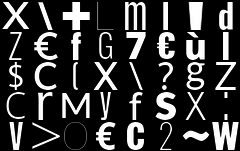
\includegraphics[width=0.3\textwidth]{images/dataset-symbols.png}
	\caption{Esempio di simboli singoli del dataset.}
	\label{fig:dataset-symbols}
\end{figure}

\subsection{Permutazioni di margini}

Come menzionato precedentemente, il modello di classificazione utilizza, oltre al bounding box del simbolo, anche i margini superiore e inferiore del simbolo rispetto al bounding box globale dell'intera parola. Per questo motivo è necessario che il dataset contenga questa informazione per far sì che il modello possa apprendere le relazioni tra il simbolo e il bounding box globale.
\\ \\
L'approccio utilizzato è il seguente, per ogni font:
\begin{itemize}
	\item Si scelgono dimensione di font e quadro dell'immagine arbitrari, font sufficientemente piccolo e quadro abbastanza grande da consentire a qualsiasi simbolo stampato di entrare all'interno dell'immagine.
	\item Si genera un'immagine quadrata per ogni simbolo, con il simbolo centrato all'interno dell'immagine.
	\item Si calcolano, per ogni simbolo, i margini superiore e inferiore del simbolo rispetto al quadro dell'immagine.
	\item Si normalizzano i margini rispetto all'altezza del quadro dell'immagine, in modo da ottenere valori compresi tra 0 e 1.
	\item Vengono create delle permutazioni dei margini, in modo che nel dataset sia presente ogni possibile combinazione di margini per ogni simbolo.
\end{itemize}

Il dataset finale conterrà quindi un simbolo per ogni font, con le varie combinazioni di margini.  Nel caso dei font considerati, il dataset contiene un totale di 179292 tuple.

È importante notare che a causa di questa ultima aggiunta il dataset dei simboli singoli non rimane perfettamente bilanciato: non tutte le classi (simboli) sono rappresentate dallo stesso numero di campioni. Ad esempio, le parentesi tonde (\texttt{(} e \texttt{)}) sono presenti con circa 600 campioni ciascuna, mentre il trattino (\texttt{-}) conta circa 5000 campioni.

Il dataset è stato suddiviso in due sottoinsiemi: train e test. La suddivisione è stata effettuata secondo una proporzione 75\% per il training e 25\% per il test, necessario per la valutazione delle prestazioni del modello.

\subsection{Struttura del dataset}

Il dataset si compone di una serie di cartelle, una per ogni font, contenenti le immagini dei simboli. Ogni cartella è denominata con il nome del font e contiene le immagini dei simboli in formato PNG. I nomi delle immagini contengono il nome del simbolo rappresentato. Sullo stesso livello della cartella del font, sono presenti due file CSV: uno per il training e uno per il test. Questi file contengono l'elenco dei campioni, con la seguente struttura:
\begin{center}
(font, immagine, simbolo, margine\_superiore (\%), margine\_inferiore (\%))
\end{center}

\section{Dataset degli screenshot}
\label{sec:dataset_screenshots}

Il dataset degli screenshot è stato creato per testare l'intera pipeline, dalla suddivisione in caratteri alla classificazione del singolo carattere. Il suo unico scopo è quello di testare l'accuratezza della pipeline per poterne valutare le prestazioni. 

Il dataset contiene immagini di screenshot contenenti una sequenza di 10 simboli casuali. In aggiunta ai simboli considerati nel dataset dei simboli singoli, sono stati aggiunti i caratteri "spazio" e "virgolette" (`"`), in modo da poter testare le euristiche relative al riconoscimento di questi caratteri.

Per la generazione di ogni immagine viene utilizzato un approccio simile a quello utilizzato per il dataset dei simboli singoli. Viene utilizzato Pillow per generare gli screenshot sintetici, scegliando un font casuale e stampando al suo interno la sequenza di simboli da testare.
Per aumentare la precisione delle metriche, vengono inoltre selezionati dei colori casuali per il testo e lo sfondo, in modo da simulare screenshot reali e verificare che le operazioni di pre-processing siano efficaci.

Sono state previste due varianti del dataset, in modo da poter testare la pipeline in modo più completo e verificare che le euristiche implementate funzionino correttamente.

\begin{itemize}
	\item \textbf{Sequenze di 10 simboli casuali}: prevede immagini di sequenze di 10 caratteri estratti randomicamente e concatenati per formare una parola (o una frase, considerando che lo spazio è incluso tra i simboli stampati).
	\item \textbf{Frasi di senso compiuto}: contiene immagini di screenshot di frasi di senso compiuto, estratte da un dataset pubblico di citazioni in lingua inglese. In particolare, le frasi sono state selezionate da un dataset pubblico disponibile su Hugging Face \footnote{Abir ELTAIEF, \textit{english\_quotes (Revision \texttt{7b544c4})}, 2023. Disponibile su: \url{https://huggingface.co/datasets/Abirate/english_quotes}, DOI: 10.57967/hf/1053.}
\end{itemize}



